\documentclass[journal]{IEEEtran}
\usepackage[a5paper, margin=10mm]{geometry}
%\usepackage{lmodern} % Ensure lmodern is loaded for pdflatex
\usepackage{tfrupee} % Include tfrupee package


\setlength{\headheight}{1cm} % Set the height of the header box
\setlength{\headsep}{0mm}     % Set the distance between the header box and the top of the text


%\usepackage[a5paper, top=10mm, bottom=10mm, left=10mm, right=10mm]{geometry}

%
\setlength{\intextsep}{10pt} % Space between text and floats

\makeindex


\usepackage{cite}
\usepackage{amsmath,amssymb,amsfonts,amsthm}
\usepackage{algorithmic}
\usepackage{graphicx}
\usepackage{textcomp}
\usepackage{xcolor}
\usepackage{txfonts}
\usepackage{listings}
\usepackage{enumitem}
\usepackage{mathtools}
\usepackage{gensymb}
\usepackage{comment}
\usepackage[breaklinks=true]{hyperref}
\usepackage{tkz-euclide} 
\usepackage{listings}
\usepackage{multicol}
\usepackage{xparse}
\usepackage{gvv}
%\def\inputGnumericTable{}                                 
\usepackage[latin1]{inputenc}                                
\usepackage{color}                                            
\usepackage{array}                                            
\usepackage{longtable}                                       
\usepackage{calc}                                             
\usepackage{multirow}                                         
\usepackage{hhline}                                           
\usepackage{ifthen}                                               
\usepackage{lscape}
\usepackage{tabularx}
\usepackage{array}
\usepackage{float}
\usepackage{ar}
\usepackage[version=4]{mhchem}


\newtheorem{theorem}{Theorem}[section]
\newtheorem{problem}{Problem}
\newtheorem{proposition}{Proposition}[section]
\newtheorem{lemma}{Lemma}[section]
\newtheorem{corollary}[theorem]{Corollary}
\newtheorem{example}{Example}[section]
\newtheorem{definition}[problem]{Definition}
\newcommand{\BEQA}{\begin{eqnarray}}
\newcommand{\EEQA}{\end{eqnarray}}

\theoremstyle{remark}


\begin{document}
\bibliographystyle{IEEEtran}
\onecolumn

\title{2.4.26}
\author{Josyula G S Avaneesh- EE25BTECH11030}
\maketitle


\renewcommand{\thefigure}{\theenumi}
\renewcommand{\thetable}{\theenumi}
\textbf{Question}Check whether (5,-2), (6,4) and (7,-2) are the vertices of an isosceles triangle.\\
\textbf{Solution: }Given details:
\begin{align}
    \vec{A}=\myvec{5 \\ -2}\, \vec{B}=\myvec{6 \\ 4}\, \vec{C}=\myvec{7\\-2}
\end{align}
\textbf{Property:} In an isosceles triangle, the perpendicular bisector of a side passes through the opposite vertex.

\begin{align}
\vec{A}=\myvec{5 \\ -2}, \vec{B}=\myvec{6 \\ 4}, \vec{C}=\myvec{7\\-2}
\end{align}
\text{Midpoint of side } $\vec{AC}$: 
\begin{align}
 \vec{M} = \frac{\vec{A}+\vec{C}}{2} 
= \frac{\myvec{5\\-2}+\myvec{7\\-2}}{2} 
= \myvec{6\\-2}
\end{align}
\text{Direction vector of side } $\vec{AC}$: 
\begin{align}
 \vec{C}-\vec{A} = \myvec{7\\-2}-\myvec{5\\-2} 
= \myvec{2\\0}
\end{align}
\text{Vector from midpoint $\vec{M}$ to } $\vec{B}$:
\begin{align}
\vec{B}-\vec{M} = \myvec{6\\4}-\myvec{6\\-2} 
= \myvec{0\\6}
\end{align}
\begin{align}
(\vec{C}-\vec{A})^\top(\vec{B}-\vec{M}) 
= \myvec{2&0}\myvec{0\\6} = 2(0)+0(6)=0
\end{align}
\begin{align*}
 \vec{B} \text{ lies on the perpendicular bisector of side } \vec{AC}.\\
 \therefore \vec{AB} = \vec{BC} \implies \triangle ABC \text{ is isosceles.}
\end{align*}

\begin{figure}[H]
    \centering
    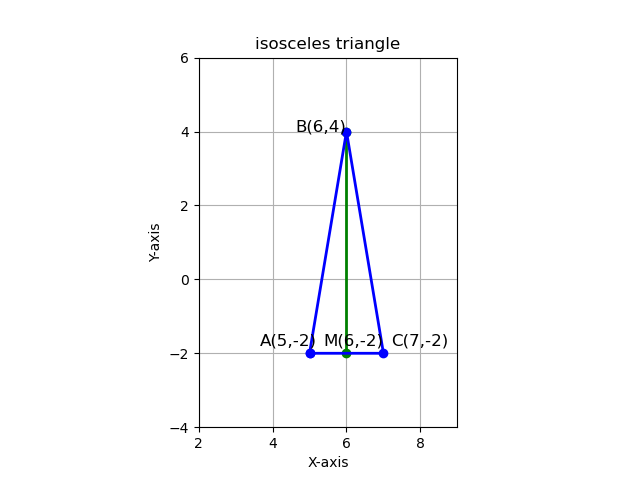
\includegraphics[width=1\columnwidth]{figs/triangle2.png}
    \caption{isosceles triangle}
    \label{fig:placeholder_1}
\end{figure}
\end{document}